En esta sección se describe la construcción física de cada uno de los sistemas que conforman el proyecto. Así mismo, se describen los cambios realizados al diseño planteado en Trabajo Terminal I, ya que, al trabajar la construcción de la estructura fue necesario realizar modificaciones al diseño planteado originalmente debido a limitaciones en cuanto a disponibilidad de recursos materiales, herramientas y limitaciones de tiempo, así como a factores no previstos en el diseño mecánico. A continuación se describen dichas modificaciones y se realizan pruebas para verificar el funcionamiento de cada sistema. 
%\section{Hoja de especificaciones del usuario}
%\label{sec:hoja_usuario}
%El sistema de ortesis robótica está diseñado para un rango de usuarios que cumpla con las siguientes características antropométricas, obtenidas de estudios de población mexicana \cite{TT2_01}, \cite{TT2_02}:
%
%\begin{table}[h!]
%	\centering
%	\caption{Hoja de especificaciones antropométricas (resumen).}
%	\begin{tabular}{|l|c|c|c|c|c|}
%		\hline
%		\textbf{Parámetro} &\textbf{Unidad} & \textbf{ID} & \textbf{P5} & \textbf{P95} & \textbf{Mín / Máx (diseño)} \\
%		\hline
%		Longitud total de pierna	 & cm &1&81 & 94 & 81-94 $\pm$ 10mm \\ \hline
%		Longitud a altura rodilla	 & cm &2& 43.4 & 52.6 & 43.4-52.6 $\pm$ 10mm \\ \hline
%		Perímetro pantorrilla 		 & cm &3& 31.5 & 42 & 31.5-42 $\pm$ 10mm \\ \hline
%		Altura sentado 				 & cm &4& 82.5 & 95 & 82.5-95 $\pm$ 10mm \\ \hline
%		Longitud nalga-poplíteo 	 & cm &5& 43.2 & 52.6 & 43.2-52.6 $\pm$ 10mm \\ \hline
%		Longitud nalga-rodilla 		 & cm &6& 53.7 & 64 & 53.7-64 $\pm$ 10mm \\ \hline
%		Altura poplítea				 & cm &7& 37.4 & 45.3&37.4-45.3 $\pm$ 10mm\\ \hline
%		Altura rodilla sentado		 & cm &8&47.3&55.6&47.3-55.6 $\pm$ 10mm\\ \hline
%		Anchura codos				 & cm &9& 44.3 & 62 & 44.3-62 $\pm$ 10mm \\ \hline
%		Anchura cadera (sentado) 	 & cm &10& 32.8 & 42.3 & 32.8-42.3 $\pm$ 10mm \\ \hline
%		Peso corporal (P95) 		 & kg && 55 & 97.3 & \textbf{Carga diseño = 92} \\
%		\hline
%	\end{tabular}
%\end{table}
%\begin{figure}[h!]
%	\centering
%	\includegraphics[width=0.2\textwidth]{figure/P06.png}
%	\caption[Dimensión antropométrica de longitud de pierna.]{Dimensión antropométrica de longitud de pierna.\label{fig:P06}}
%\end{figure}
%\begin{figure}[h!]
%	\centering
%	\subcaptionbox{Longitud a altura de rodilla y perímetro de pantorrilla.\label{fig:P07}}
%	{\includegraphics [trim = 0 0cm 0 0, clip,width=8cm]{figure/P07.png}}\\
%	\subcaptionbox{Longitudes y alturas en posición sentado.\label{fig:P08}}
%	{\includegraphics [trim = 0 0cm 0 0, clip,width=8cm]{figure/P08.png}}
%	\caption[Dimensiones antropométricas contempladas para diseño del sistema.]{Dimensiones antropométricas contempladas para diseño del sistema.\label{fig:P07P08}}
%\end{figure}
%Estas dimensiones determinan:
%\begin{itemize}
%	\item La distancia y ajuste de los puntos de sujeción mecánica.
%	\item La fuerza nominal requerida de los actuadores lineales y rotativos.
%	\item La configuración de las rutinas de movimiento, para mantener seguridad y comodidad.
%\end{itemize}
%
%El diseño mecánico y los mecanismos de sujeción (véase Anexo \ref{sec:planos de manufactura}, \nameref{sec:planos de manufactura}) se dimensionaron considerando el percentil 95 para garantizar compatibilidad con la mayoría de los usuarios.
%\clearpage
%\subsection{Adquisición y verificación de componentes}\label{subsec:adquisicion}
%Parte importante para la construcción del proyecto recayó en la adquisición de los componentes a utilizar, tomando en cuenta su capacidad para desempeñar su función esperada, así como los tiempos de envío y entrega una vez realizados los pedidos.
%%% DESCRIBIR LO QUE SE COMPRÓ CON BASE EN LA LISTA DE MATERIALES EN LA TABLA DE COSTOS
%\subsubsection{Gestión de proveedores y materiales}\label{subsubsec:gestion_proveedores}
%La fase de implementación dio inicio con la adquisición de los componentes y materiales estructurales definidos en el diseño detallado desarrollado en Trabajo Terminal I. La selección de los componentes se basó en el cumplimiento de las especificaciones técnicas, mientras que para la selección de proveedores  se tomó en cuenta la disponibilidad en el mercado nacional, costos y tiempos de entrega.
%\begin{figure}[h!]
%	\centering
%	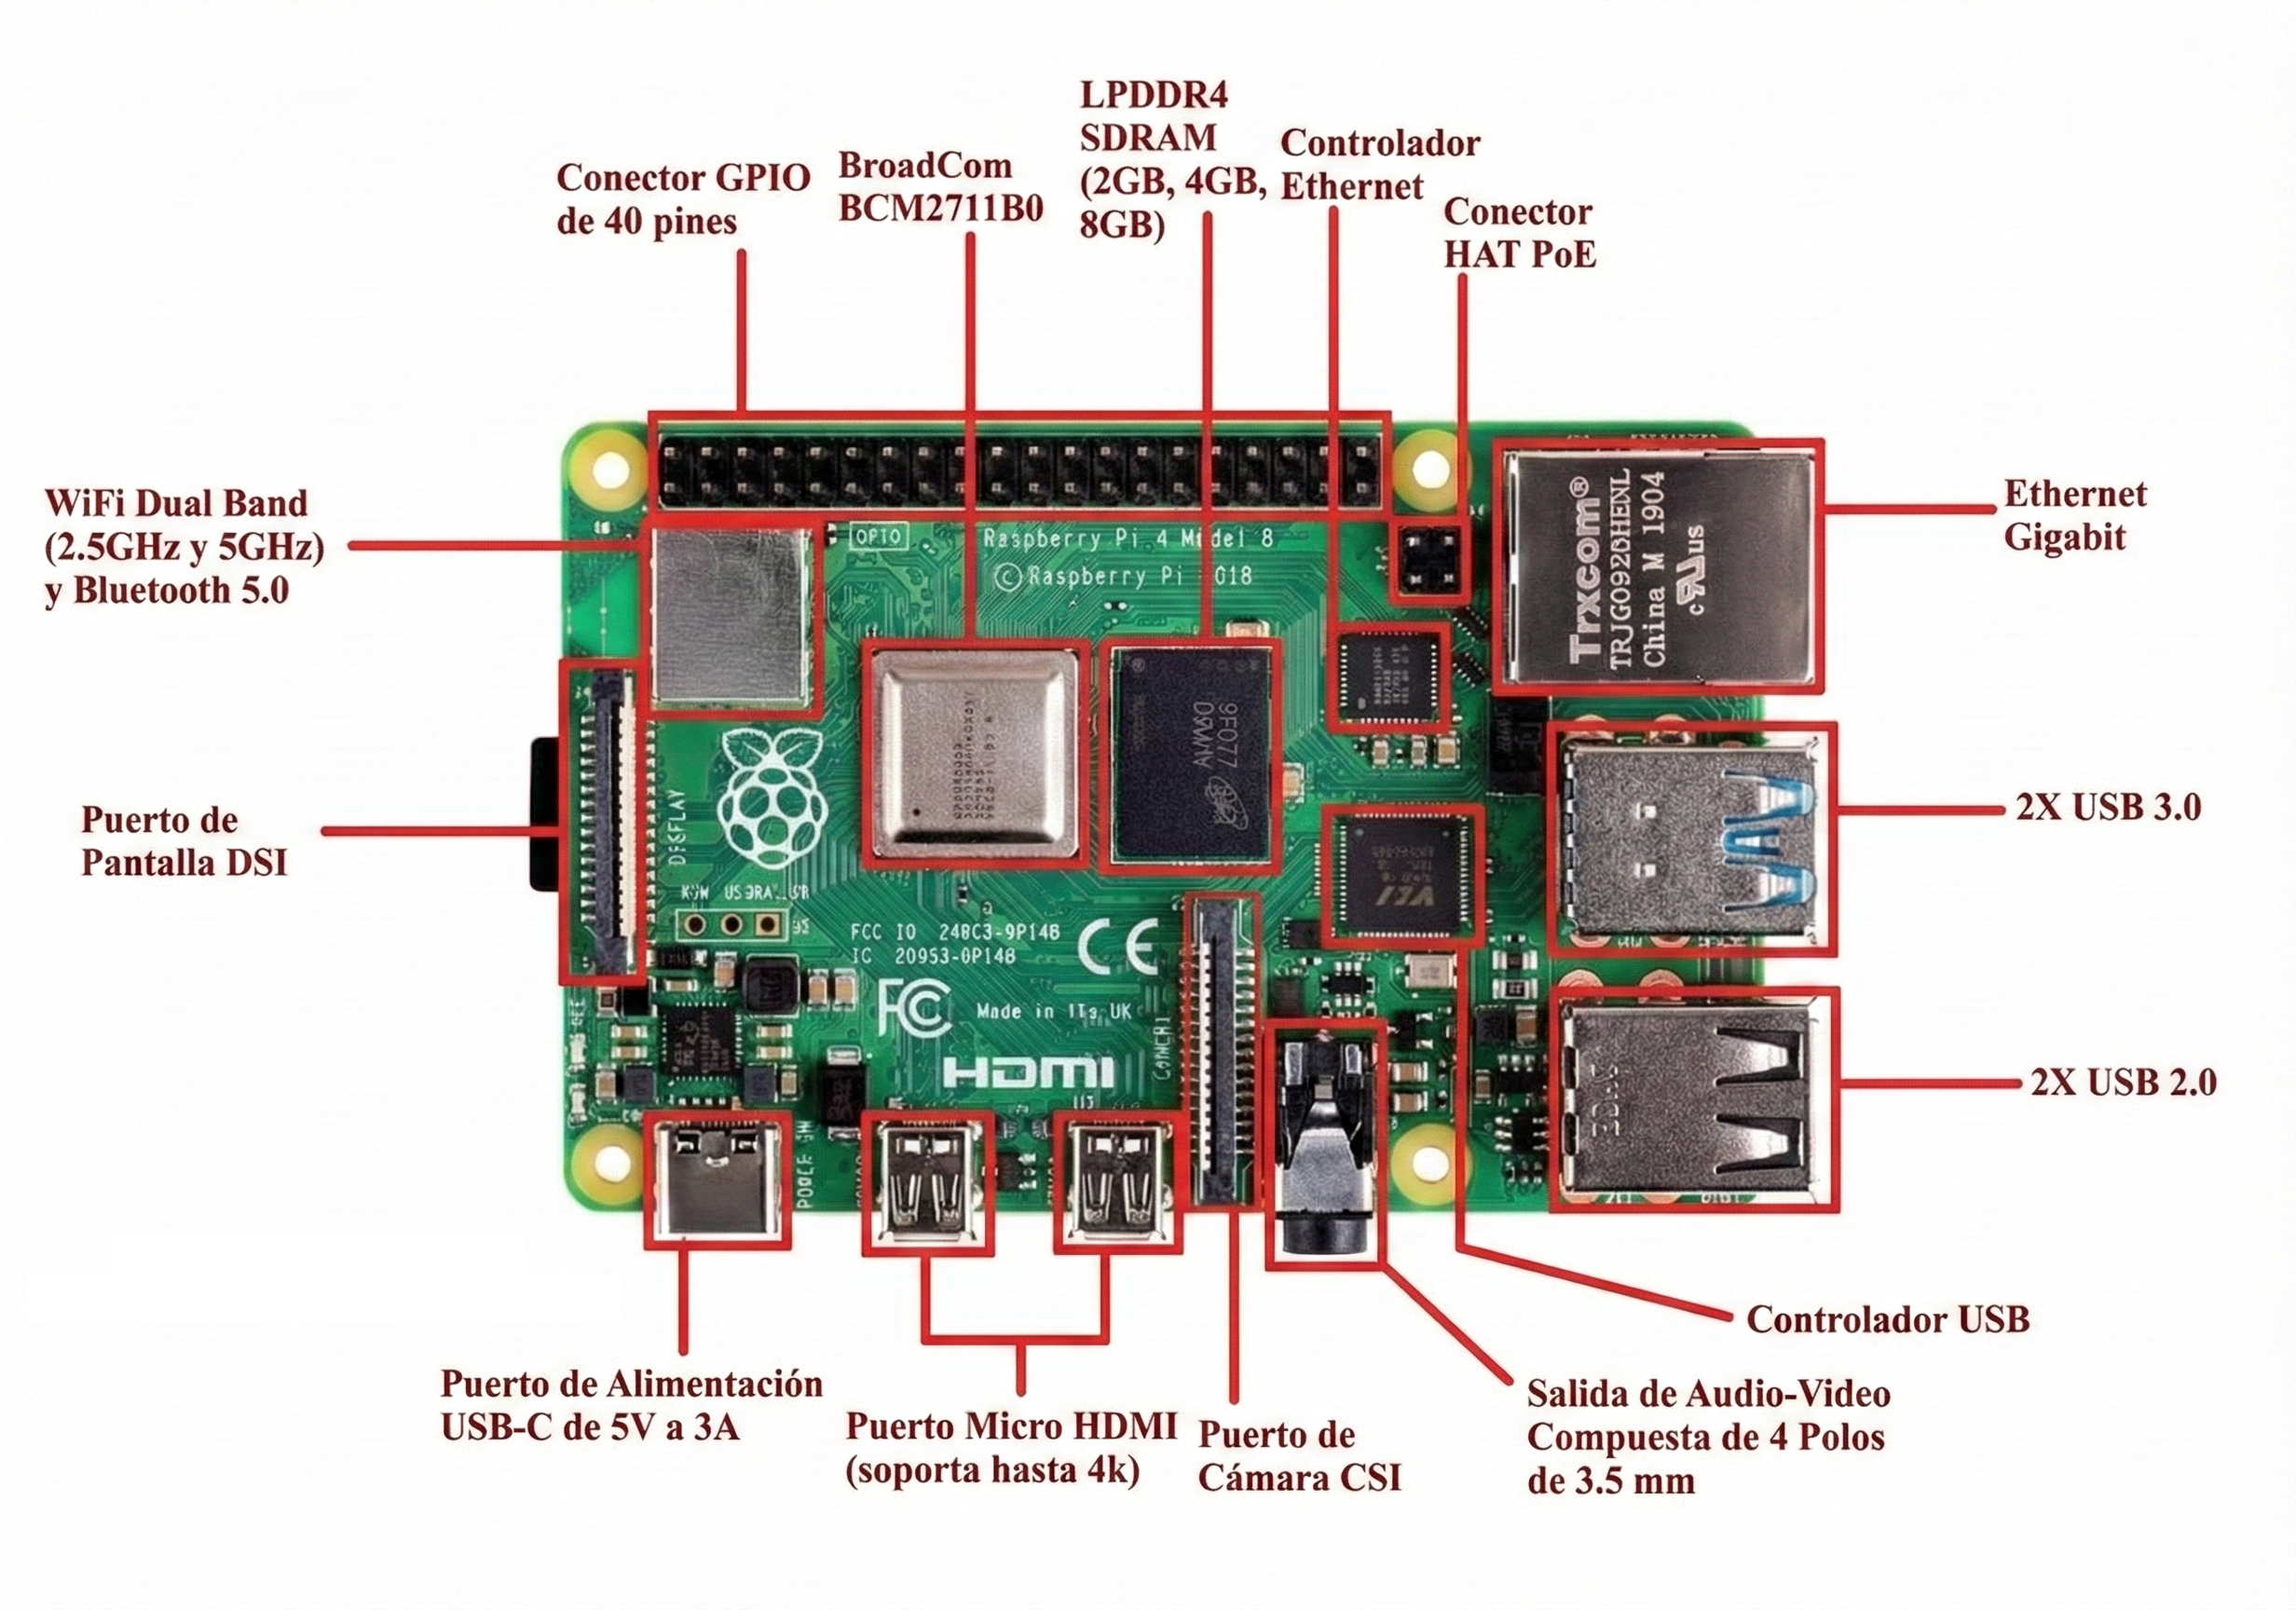
\includegraphics[width=0.7\textwidth]{figure/S7_control/Raspberry_pi4_pines.png}
%	\caption{Distribución de pines en la unidad de procesamiento Raspberry Pi 4.\label{fig:comp_waveshare}}
%\end{figure}
%
%Se gestionó la compra de todos los elementos, desde los perfiles estructurales PTR y de aluminio, hasta los componentes necesarios como los drivers \texttt{HSS57} y \texttt{HSS86}, los motores a pasos Nema 23 y Nema 34, y la unidad de procesamiento (Raspberry Pi 4) como componente crítico para el sistema de control a través del cual se coordinan los sistemas de comunicación y sistemas de movimiento. En la Fig. \ref{fig:comp_waveshare} se muestra la distribución de los pines en la unidad de procesamiento Raspberry Pi4.
%%\subsection{Inspección de componentes críticos}\label{subsec:inspeccion_componentes}
%%Una vez recibidos los materiales, se realizó una inspección visual y técnica para verificar que correspondieran a las especificaciones requeridas para el proyecto.
%%
%%Se verificó que la unidad de procesamiento [Fig. \ref{fig:comp_rpi}] corresponde al modelo Raspberry Pi 4 Model B con 4GB de RAM. Para la HMI, se recibió la pantalla táctil Waveshare de 7 pulgadas [Fig. \ref{fig:comp_waveshare}], confirmando su compatibilidad de conexión HDMI y USB. Los sensores y los interruptores de límite fueron inspeccionados visualmente. 
% 
%%\begin{figure}[h!]
%%	\centering
%%	\subcaptionbox{Distribución de pines en la unidad de procesamiento Raspberry Pi 4.\label{fig:comp_rpi}}
%%	{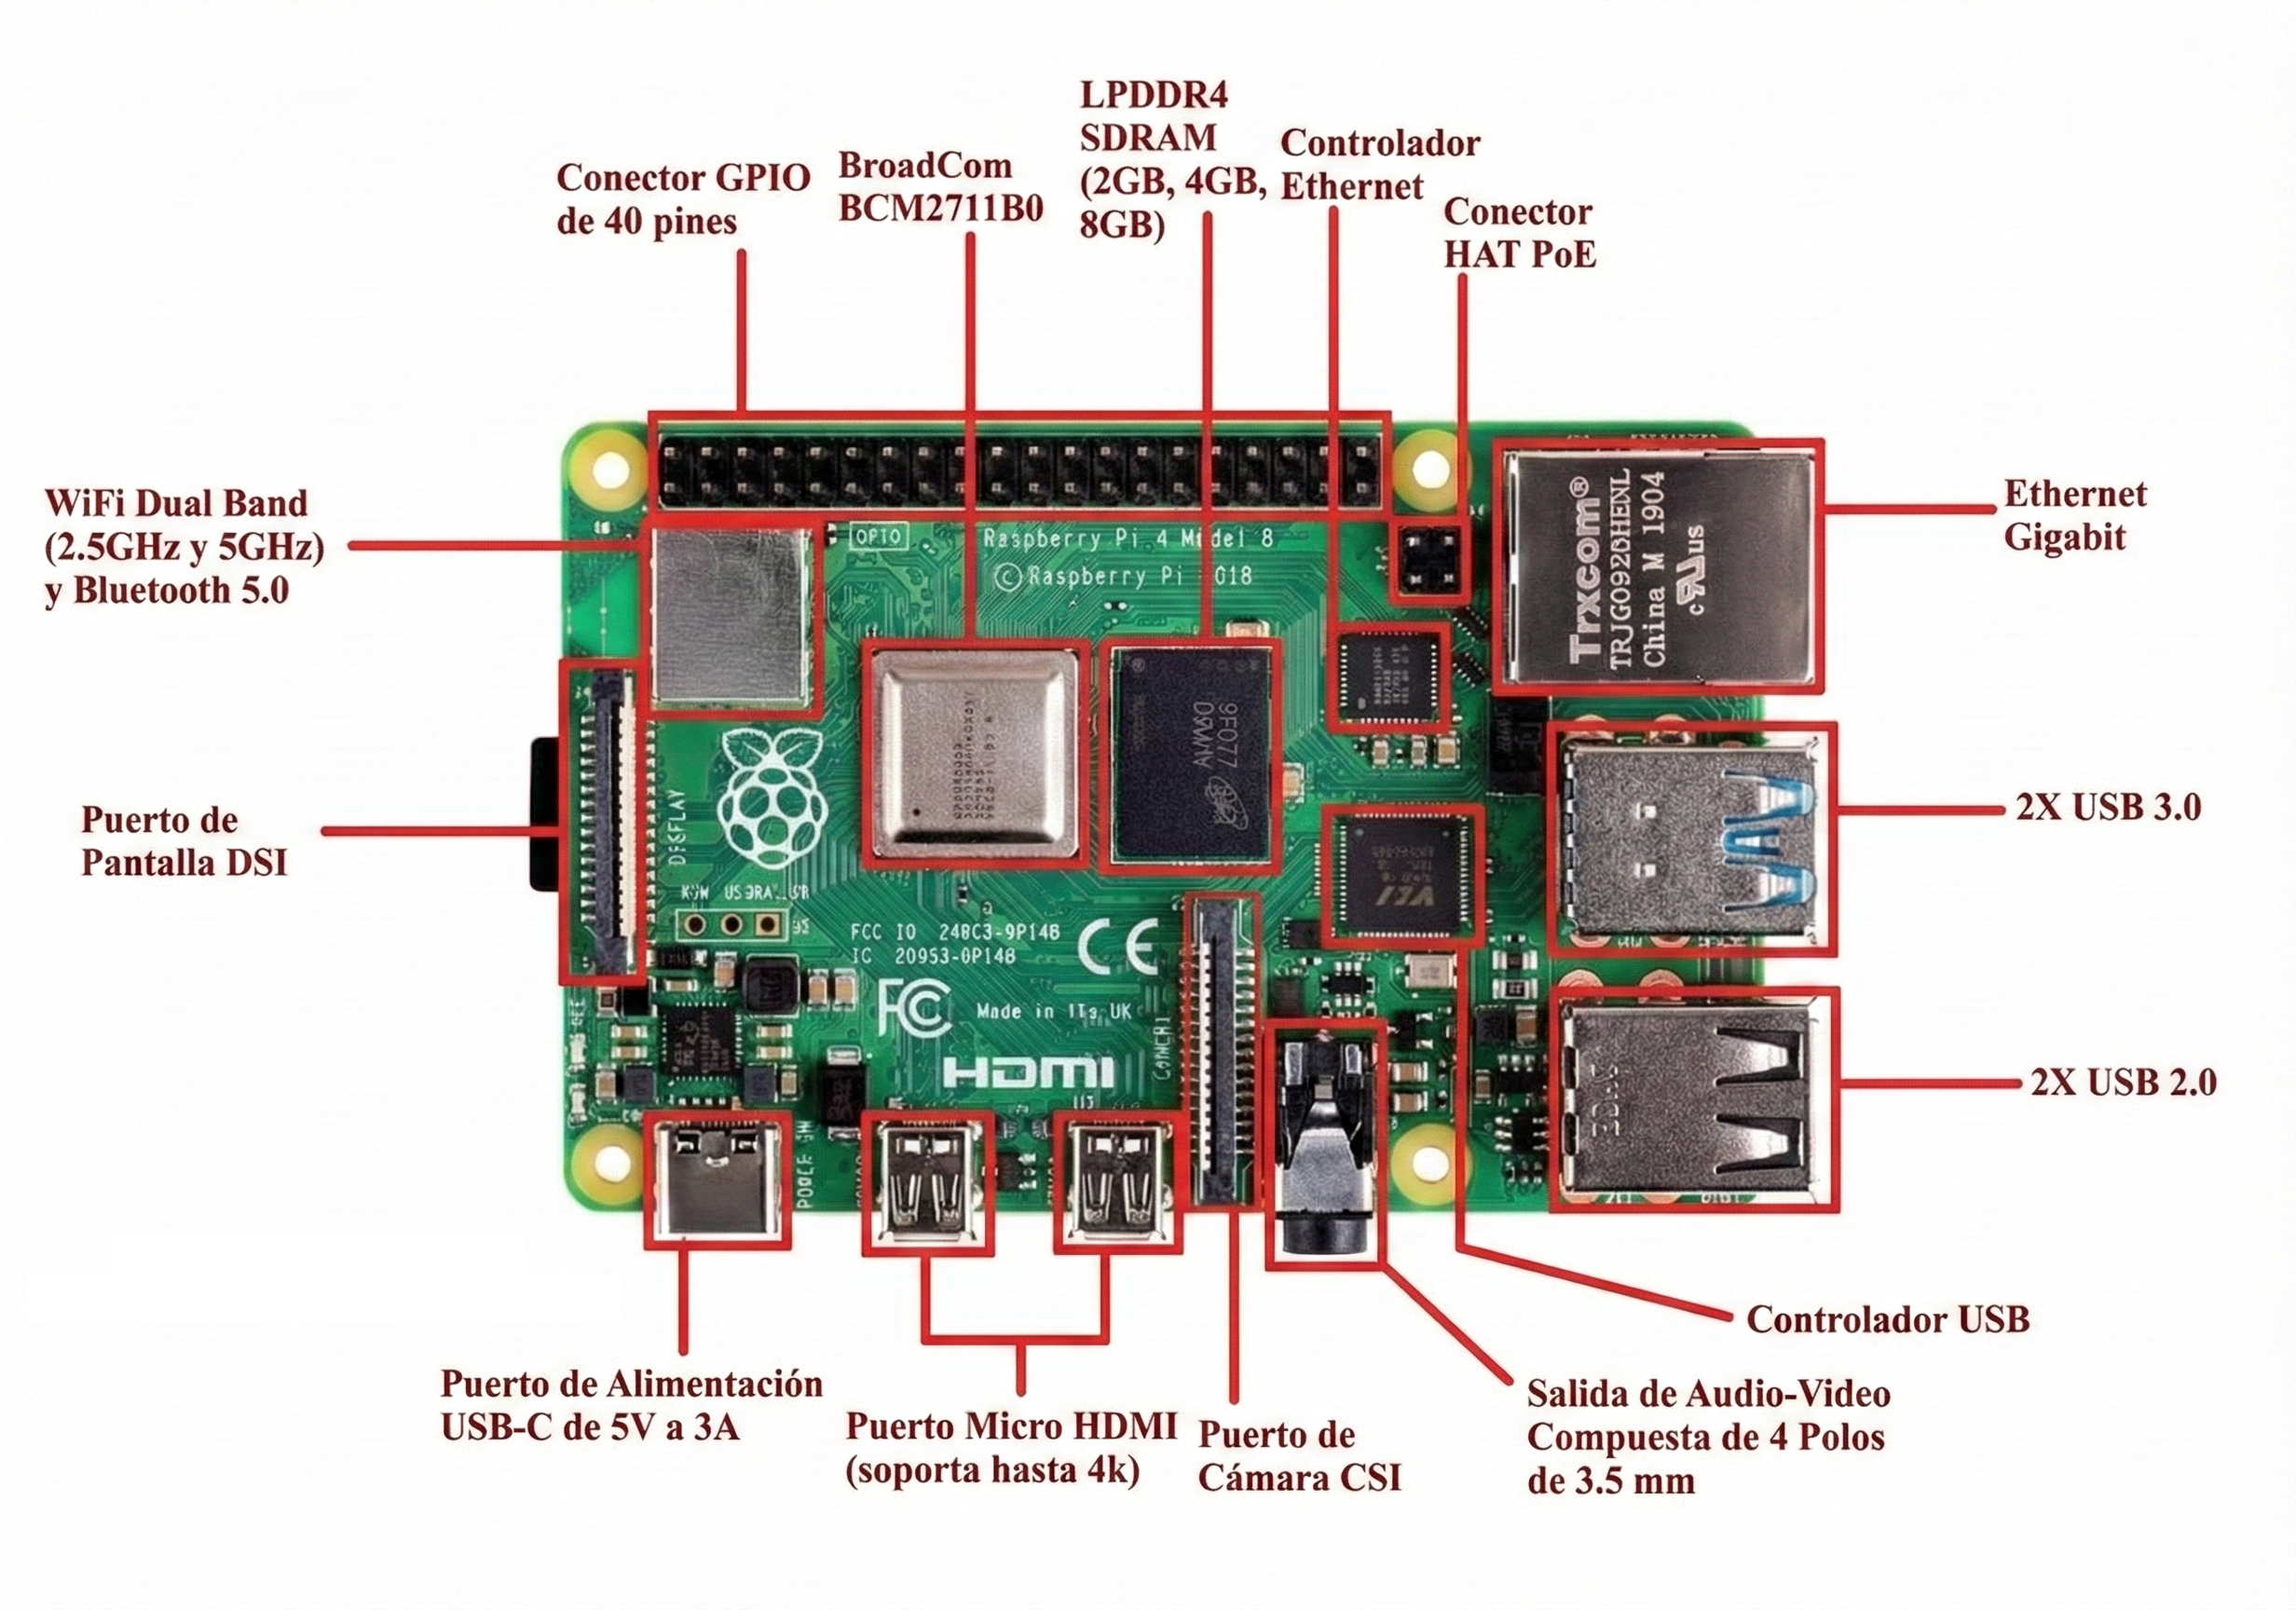
\includegraphics[width=0.6\textwidth]{figure/S7_control/Raspberry_pi4_pines.png}}
%%	\subcaptionbox{Pantalla HMI Waveshare de 7 pulgadas.\label{fig:comp_waveshare}}
%%	{\includegraphics[width=0.48\textwidth]{figure/s6_hmi/Waveshare.png}}
%%	\caption{Componentes principales del sistema de control y comunicación.}
%%\end{figure}


\section{Sistema estructural (S1)}\label{Implementacion S1}
La construcción del sistema estructural fue dividido en secciones comenzando por la base de la cama que soportaría a los mecanismos de flexión-extensión, abducción-aducción, así como el montaje de componentes electrónicos y actuadores requeridos para los sistemas de control, seguridad eléctrica y comunicación humano-máquina.
\subsection{Modificaciones al diseño del sistema estructural}
Al construir la placa de acople para el mecanismo de flexión-extensión se encontró que la placa de acero tenía una superficie de $89,420\ mm^2$ que no tenía contacto con el mecanismo, por lo que se optó por recortar la placa con la finalidad de reducir el par torsor generado sobre el eje. Además, se optó por soldar directamente la placa al eje sin aletas. En la Fig. \ref{fig:placa acople b modificacion} se muestra el antes y después de la modificación realizada en el diseño.
\begin{figure}[h!]
	\centering
	\subcaptionbox{Forma de la placa de acople original.}
	{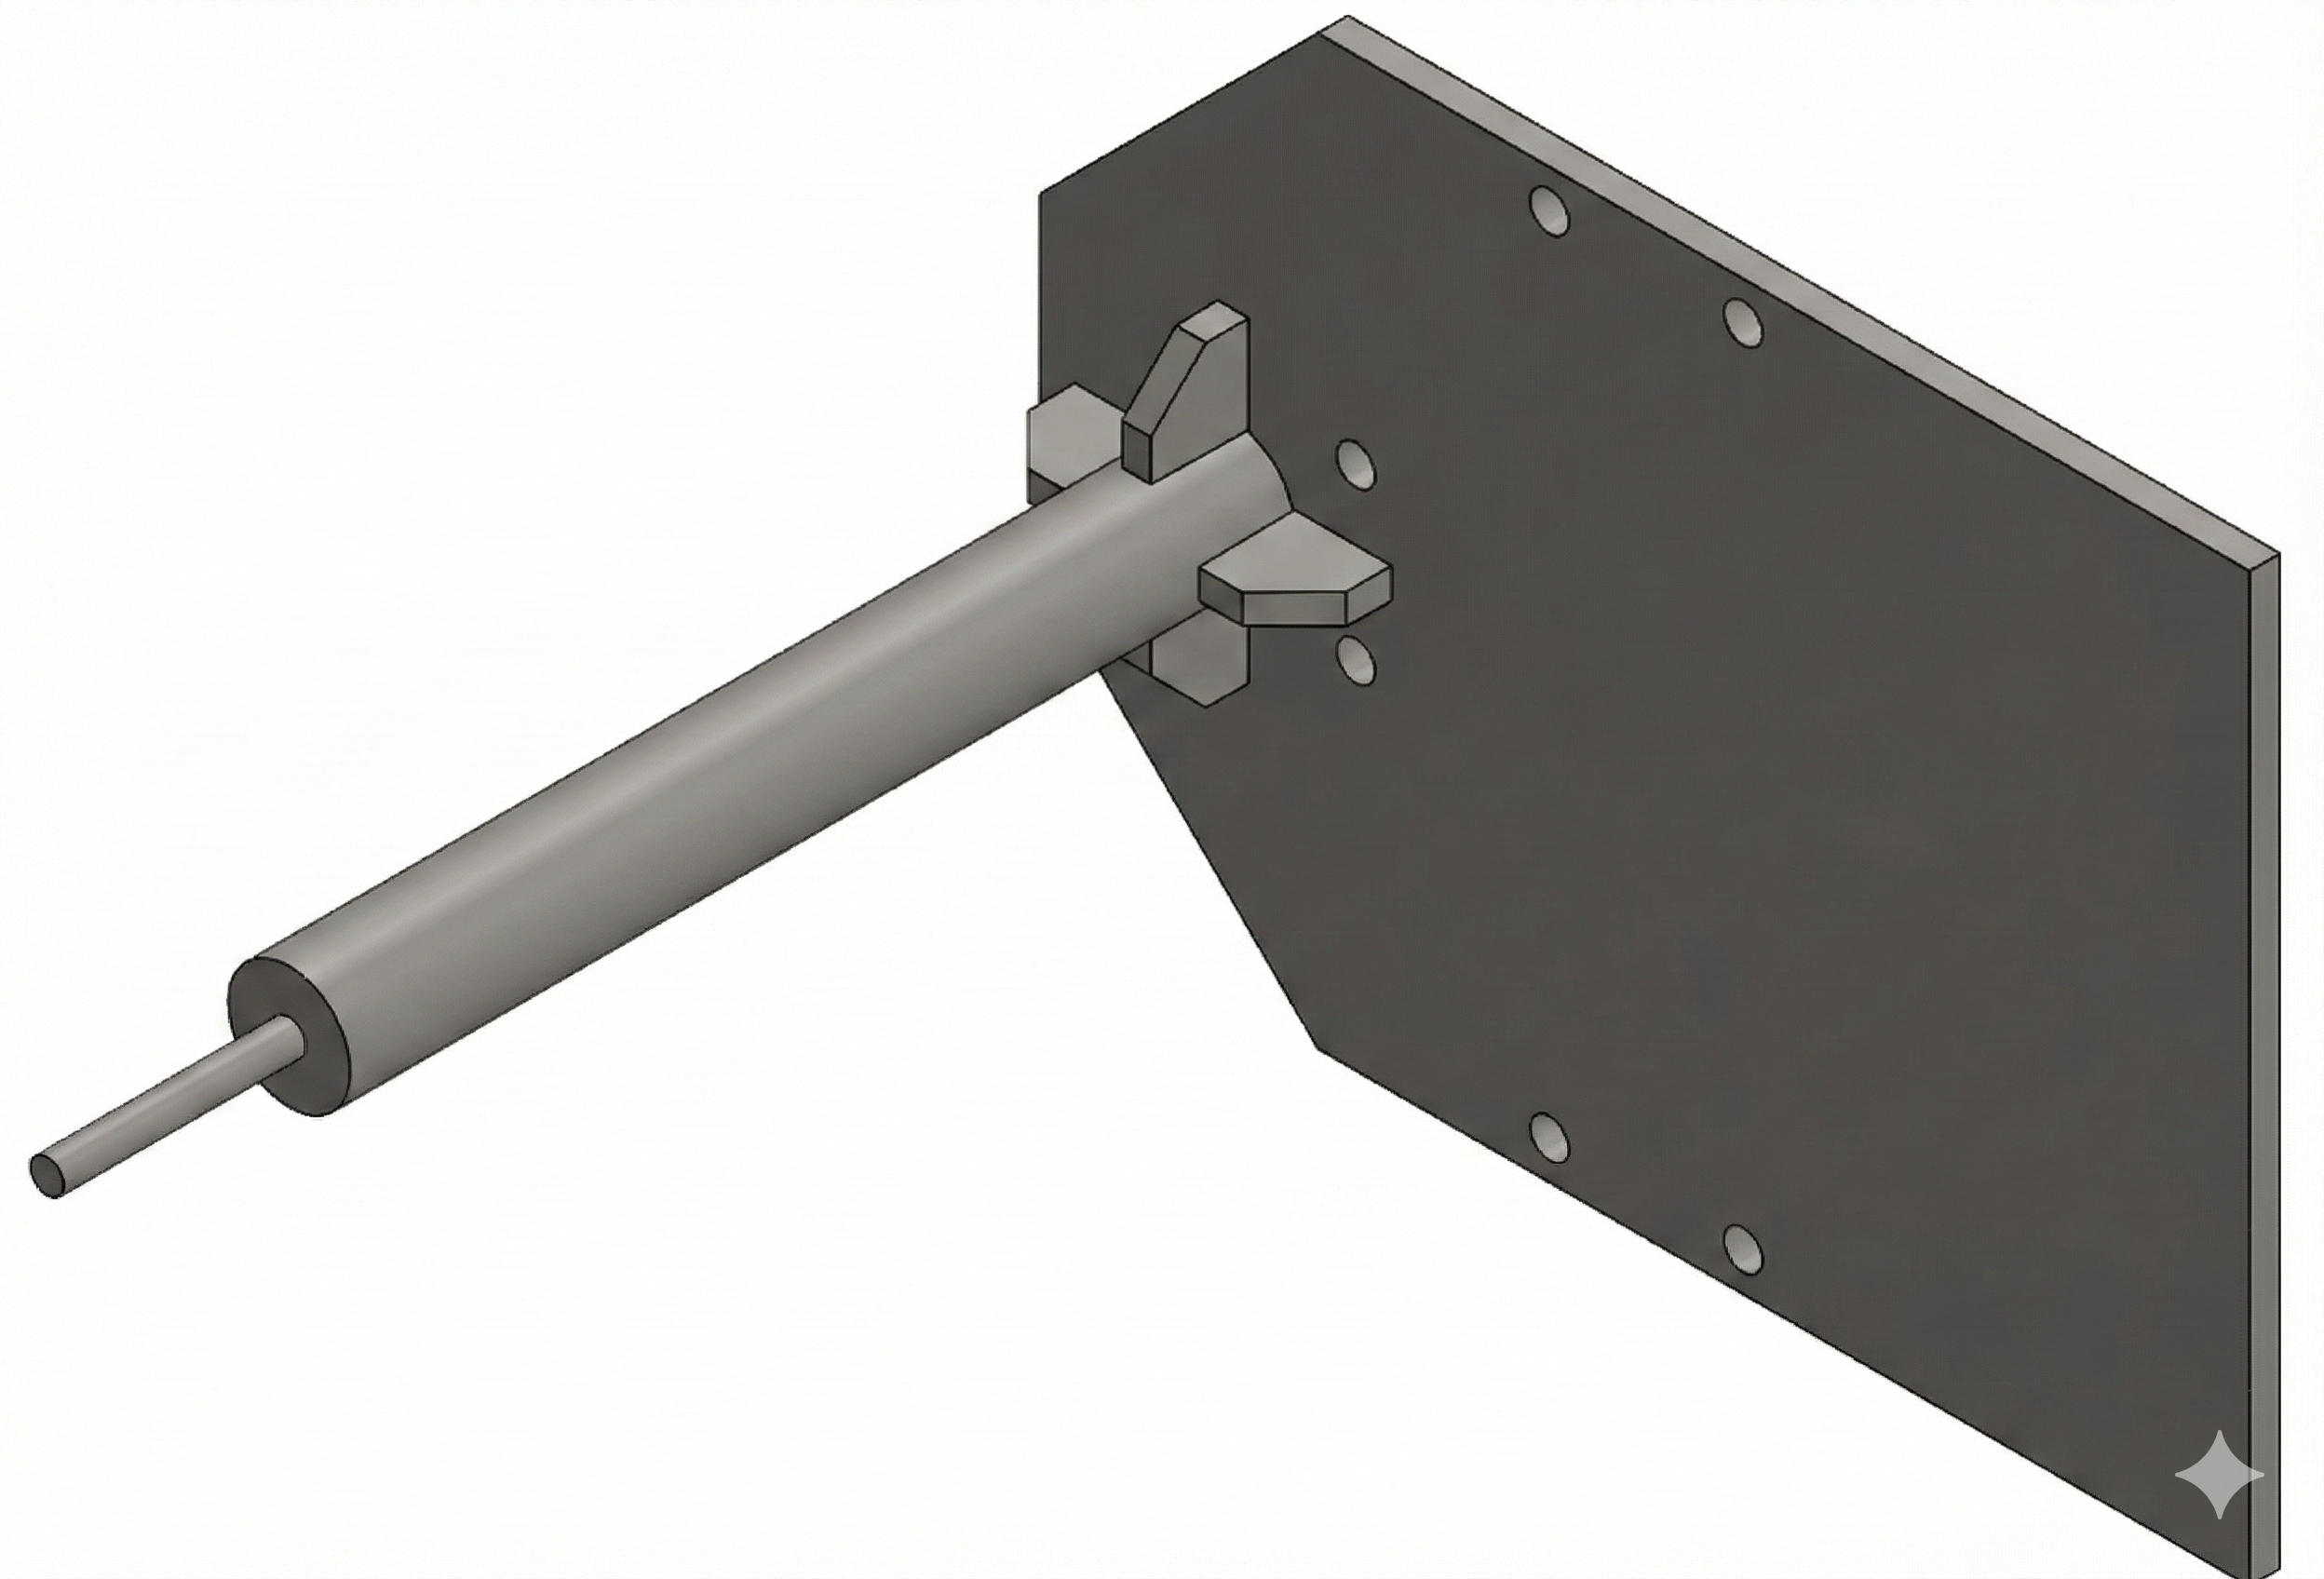
\includegraphics [trim = 0 0cm 0 0, clip,width=7cm]{figure/img_estructura/Placa acople B original.png}}
	\subcaptionbox{Forma de la placa de acople modificada.}
	{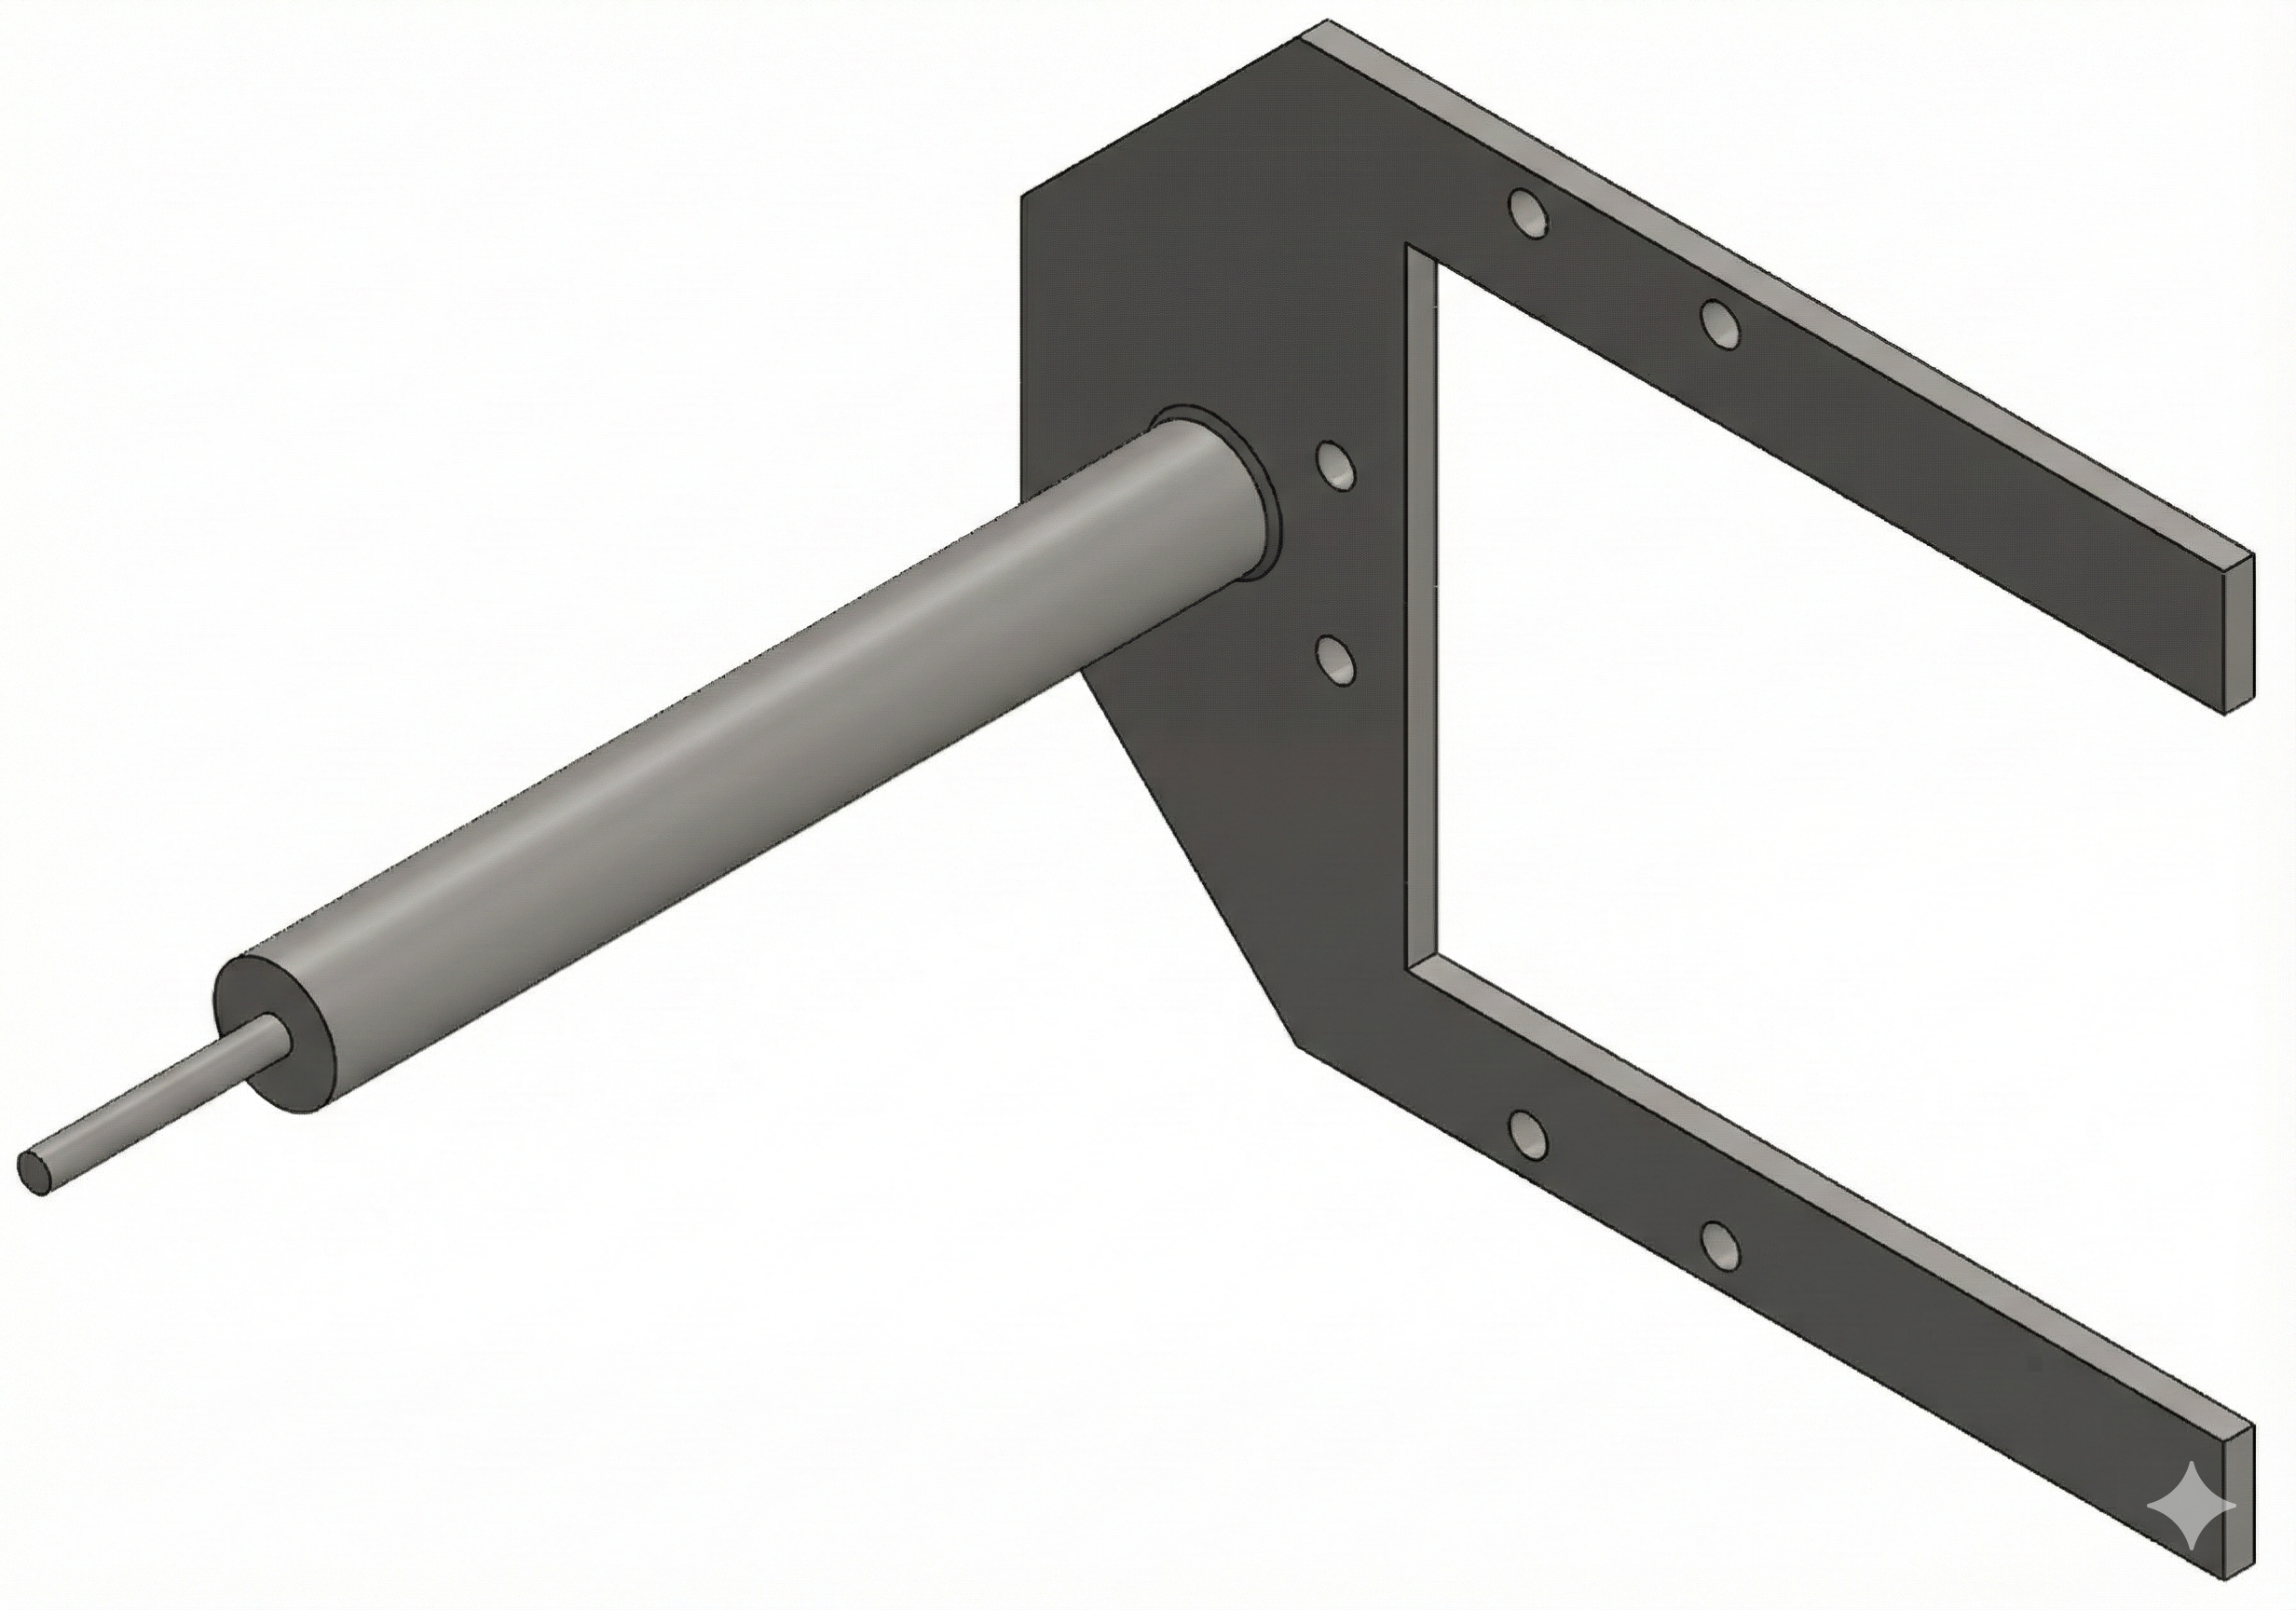
\includegraphics [trim = 0 0cm 0 0, clip,width=7.3cm]{figure/img_estructura/Placa acople B modificada.png}}
	\caption{Modificación en el diseño de la placa de acople para el mecanismo de flexión-extensión.\label{fig:placa acople b modificacion}}
\end{figure}
\subsection{Construcción de la cama de soporte}
El soporte principal se construyó utilizando perfiles PTR soldados con la finalidad de obtener una base rígida ante la carga vertical del paciente y los mecanismos que soportará la estructura. En la Fig. \ref{fig:perfil_ptr} se muestra el perfil del PTR con dimensiones 2x2 pulgadas y grosor de calibre 12. 

 \begin{figure}[h!]
 	\centering
 	\includegraphics[width=0.4\textwidth]{figure/img_estructura/PTR_perfil_.png}
 	\caption{Perfil PTR de dimensión 2x2 pulgadas y calibre 12, para construcción de la cama soporte.\label{fig:perfil_ptr}}
 \end{figure}
Se colocó una placa de triplay con un espesor de 15 mm sobre la base del soporte principal acorde a su forma y dimensiones, y sobre esta placa se integró una colchoneta de espuma de alta densidad que se utiliza como superficie de acojinamiento para comodidad del paciente con un espesor de 45 mm [Fig. \ref{fig:cama_estructura}]. %La elevación de la placa de triplay y la colchoneta permiten alinear el eje de rotación de la articulación coxofemoral del paciente con el eje mecánico del actuador de abducción. Sin este ajuste de altura la discrepancia de alturas generaría un par de fuerzas no deseado en la cadera del paciente durante la sesión. 36.3 110 
\begin{figure}[h!]
	\centering
	\includegraphics[width=0.48\textwidth]{figure/img_estructura/Colchoneta_triplay.png}
	\caption{Implementación física con colchoneta y placa de triplay sobre la base del sistema estructural.\label{fig:cama_estructura}}
\end{figure}
\subsection{Construcción del mecanismo de flexión-extensión}
El mecanismo se manufacturó utilizando perfiles de aluminio 6061-T6 para reducir la dificultad del movimiento relacionada con la inercia del mecanismo. El mecanismo se conforma de una parte ajustable para poder acoplar la pierna del paciente y realizar el movimiento de flexión-extensión; y una segunda parte estática de dimensiones fijas que actúan como soporte para la parte móvil ajustable. En la Fig. \ref{fig:mecanismo_flexion_extension_raw} se observan las partes del mecanismo, así como las dimensiones fijas de la parte estática.

Las uniones que integran la parte ajustable del mecanismo son las uniones Clevis, las cuales fueron seleccionadas por medio de matrices de decisión en la fase de diseño. Se utilizó tornillería de acero galvanizado para dichas uniones. En la Fig. \ref{fig:union_coxofemoral} y en la Fig. \ref{fig:union_rodilla} se muestran las uniones en la articulación del coxofemoral y rodilla respectivamente. 
\clearpage
\begin{figure}[h!]
	\centering
	\includegraphics[width=0.48\textwidth]{figure/img_estructura/Mecanismo_flexion_extension.png}
	\caption{Partes del mecanismo de flexión-extensión.\label{fig:mecanismo_flexion_extension_raw}}
\end{figure} 
\begin{figure}[h!]
	\centering
	\subcaptionbox{Vista lateral frontal.}
	{\includegraphics [trim = 0 0cm 0 0, clip,width=6cm]{figure/img_estructura/Union_coxo2.jpg}}
	\subcaptionbox{Vista lateral trasera.}
	{\includegraphics [trim = 0 0cm 0 0, clip,width=6cm]{figure/img_estructura/Union_coxo1.jpg}}
	\caption{Uniones Clevis en articulación de coxofemoral en mecanismo ajustable.\label{fig:union_coxofemoral}}
\end{figure}

Ambos pares de uniones Clevis fueron maquinados con aluminio 6061-T6 y soldados a los perfiles del mecanismo ajustable y estático. 
\begin{figure}[h!]
	\centering
	\subcaptionbox{Vista lateral trasera.}
	{\includegraphics [trim = 0 0cm 0 0, clip,width=6cm]{figure/img_estructura/Union_rod2.jpg}}
	\subcaptionbox{Vista superior.}
	{\includegraphics [trim = 0 0cm 0 0, clip,width=6cm]{figure/img_estructura/Union_rod3.jpg}}
	\caption{Uniones Clevis en articulación de rodilla en mecanismo ajustable.\label{fig:union_rodilla}}
\end{figure}
.
\subsubsection{Diseño de la placa base, eje de transmisión, manejo de tolerancias y deformaciones térmicas}
El mecanismo de flexión-extensión se colocó sobre una placa de acero al carbón de 1/2". La longitud de la placa fue acotada al área de transmisión de esfuerzos del actuador lineal en lugar de cubrir toda la base con la finalidad de reducir la deflexión del eje debido al peso de la pierna. Además, se implementaron múltiples puntos de apoyo (chumaceras) que fueron distribuidos a lo largo del eje de transmisión, reduciendo así el momento flector en los extremos. Sin embargo, durante el proceso de manufactura, las placas de acero fueron cortadas mediante láser. Se observó que el calor térmico generado al momento del corte provocó una curvatura, lo que dificultó el alineamiento de las placas con los rieles de la guía. Para corregir el ensamble se realizó una alineación activa, es decir, se montaron el eje, las chumaceras y la placa simultáneamente, y se ajustó la posición con esfuerzo manual antes de aplicar los puntos de soldadura y fijación final. En la Fig. \ref{fig:eje_transmision} se muestra la forma y dimensiones de la placa sobre la cual se montó la estructura de aluminio, así como sus dimensiones, así como la distribución de los componentes sobre el eje de transmisión.
\begin{figure}[h!]
	\centering
	\subcaptionbox{Forma y dimensiones de placa de acero al carbón de 1/2".}
	{\includegraphics [trim = 0 0cm 0 0, clip,width=7cm]{figure/img_estructura/placa_soporte.png}}
	\subcaptionbox{Eje de transmisión con mecanismo de flexión-extensión montado.}
	{\includegraphics [trim = 0 0cm 0 0, clip,width=7cm]{figure/img_estructura/eje_transmision.png}}
	\caption{Eje de transmisión y placa para montaje del mecanismo de flexión-extensión.\label{fig:eje_transmision}}
\end{figure}

\subsubsection{Implementación de sujeción y ajuste}
\begin{figure}[h!]
	\centering
	\includegraphics[height=0.4\textwidth]{figure/img_estructura/desplazamientos_mecanismo.png}
	\caption{Vista lateral del mecanismo de flexión-extensión.\label{fig:desplazamientos_flexion-extextension}}
\end{figure}
Para lograr la adaptabilidad a los diferentes percentiles antropométricos (P5 a P95), se implementó el sistema de ajuste telescópico en los eslabones correspondientes al fémur y la tibia, de modo que al inicio de la sesión se realice el ajuste de los tubos telescópicos a la longitud de la pierna del paciente. En la Fig. \ref{fig:desplazamientos_flexion-extextension} se muestra el mecanismo de flexión-extensión cuyos rangos de extensión son:
\begin{itemize}
	\item Extensión de tibia:
	\item Extensión de fémur:
\end{itemize} 

Para ajustar y fijar la longitud de los tubos telescópicos se emplearon tornillos tipo estrella. En la Fig. \ref{fig:tornillos_estrella} cada un tornillo por lado, sin embargo, estos fueron colocados en pares (uno en el extremo derecho y uno en el extremo izquierdo).
\begin{figure}[h!]
	\centering
	\subcaptionbox{Tornillo para tubo telescópico de fémur.}
	{\includegraphics [trim = 0 0cm 0 0, clip,width=5cm]{figure/img_estructura/tubos_teles1.jpg}}
	\subcaptionbox{Tornillo para tubo telescópico de tibia.}
	{\includegraphics [trim = 0 0cm 0 0, clip,width=5cm]{figure/img_estructura/tubos_teles2.jpg}}
	\subcaptionbox{Tornillo para ajuste de rotación del tobillo.}
	{\includegraphics [trim = 0 0cm 0 0, clip,width=5cm]{figure/img_estructura/union_tobillo.jpg}}
	\caption{Tornillos tipo estrella para sujeción y ajuste de longitud del mecanismo de flexión-extensión.\label{fig:tornillos_estrella}}
\end{figure}


\subsubsection{Discrepancias entre diseño e implementación del mecanismo de flexión-extensión}
\paragraph*{Soporte distal (pie).}
Durante el ensamble del soporte distal (pie)\footnote{Se proporciona mayor información de la manufactura de los soportes en la subsección \nameref{Implementacion S3}.}, se encontró una interferencia dimensional en la unión de la impresión 3D plegada que actúa como soporte del pie con la estructura de aluminio, por lo que se aplicó un proceso de ajuste mecánico (desbaste de 3 mm) en las caras laterales para lograr un acople deslizante.
\paragraph*{Barreno invertido en clévis (fémur).}
En uno de los tubos telescópicos del fémur, un barreno para ajustar la posición del tubo telescópico fue soldado en sentido invertido al planteado en el diseño CAD, sin embargo, no afecta al funcionamiento ni el movimiento por lo que se decidió conservar dicho cambio debido a que el funcionamiento es aceptable.

\subsection{Construcción del mecanismo de abducción-aducción.}
El mecanismo de abducción-aducción se encarga de soportar la carga del subsistema de flexión y la pierna del paciente, y produce la rotación de un eje vertical. Para este mecanismo se utilizó el motor Nema 34 acoplado un eje de acero maquinado. Sobre el eje se tienen los puntos de apoyo distribuidos que reducen el momento flector en los extremos.
\subsubsection*{Selección de elementos de rotación}
Durante la validación del diseño, se analizó la selección de los elementos rodantes para las articulaciones superior e inferior.
\begin{enumerate}
	\item \textbf{Eje inferior (carga principal):} Se implementaron chumaceras de bolas y un rodamiento axial en la base. Esto para soportar la carga axial combinada (aprox. 25 kg) con mínima fricción.
	\item \textbf{Uniones superiores (nivel coxofemoral):} Para las articulaciones superiores del mecanismo de flexión-extensión, se emplearon las juntas Clevis seleccionadas mediante tablas de decisión, la cuales no tienen rodamientos de bolas, esto se debe a que la velocidad angular de operación es muy baja ($< 0.5$ rad/s) y el ciclo de trabajo no es continuo, lo que implica que la fricción generada por el contacto metal-metal lubricado es despreciable en comparación con el par disponible de los actuadores. Además, esta configuración reduce el volumen del mecanismo en la zona de la cadera. Esto reduce el volumen ocupado por el mecanismo en la articulación coxofemoral. 
\end{enumerate}

\begin{figure}[h!]
	\centering
	\includegraphics[width=0.6\textwidth]{figure/img_componentes/Untitled.png}
	\caption{Eje principal de abducción maquinado con cuñero para acople directo al motor Nema 34.\label{fig:mecanismo_abduccion_aduccion}}
\end{figure}
\subsection{Integración de mecanismos y montaje final}
Durante las fases finales del ensamble se realizó el acoplamiento del subensamble de flexión-extensión sobre el eje de abducción, y se realizaron los barrenos para la fijación de los interruptores de límite directamente sobre la estructura, ajustando su posición para permitir el movimiento de los mecanismos de flexión-extensión y abducción-aducción. Durante este proceso se encontró fricción excesiva con partes de la estructura por lo que se recurrió al desbaste de zonas de la estructura con el fin de permitir un desplazamiento suave y evitar atascamientos. 
% Debo mencionar más sobre esta subsubsección que aún está incompleta. Agregar la referencia a la imagen donde describa como se están montando los interruptores de límite
\begin{figure}[h!]
	\centering
	\includegraphics[width=0.7\textwidth]{figure/img_componentes/Untitled.png}
	\caption{Ajuste dimensional a estructura para montaje de interruptores de límite.\label{fig:limit_switch_montaje}}
\end{figure}

\subsection{Verificación del sistema estructural}

Una vez ensamblado el sistema S1, se procedió a su validación estática antes de integrar los componentes de los sistemas de seguridad mecánica, eléctrica, controlo y comunicación.

\subsubsection{Prueba S1-01: Integridad estructural bajo carga}
\textbf{Objetivo:} Verificar que la estructura soporta la carga de diseño sin deformaciones plásticas ni fallos en las soldaduras.
\\
\textbf{Procedimiento:} Se aplicó una carga estática distribuida de 90 kg sobre la cama de soporte y una carga puntual de 20 kg sobre el mecanismo de pierna extendida, simulando el peso de un paciente en el percentil P95.
\\
\textbf{Resultados:} La estructura no presentó deformaciones visibles ni ruidos estructurales. El mecanismo de flexión mantuvo su alineación bajo carga, validando la corrección de las placas de acero.



